\subsection{Матричное представление метода контурных токов и узловых потенциалов}

\subsubsection{Топологические матрицы}

Узловая матрица [A] составляется для n-1 узла графа цепи, в ней столбца обозначают ветви, а строки - узлы.
Элемент = 1, если при выбранном направлении обхода ветвь выходит из узла, = -1, если входит, 0 если не относится.




Выделим в графе цепи остовное дерево. Хорды - ветви, не участвующие в остовном дереве.

Главные контура - контура, содержащие одну и только одну ветвь связи (хорду), нумеруются по номеру этой хорды.
Имеют направление обхода, элементы соответственно -1;1;0   против;по;не участвует. Матрица составляется аналогично и обозначается [K].
\begin{center}
	\begin{figure}[h!]
		\center{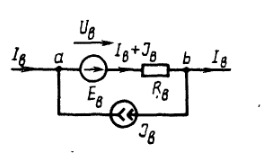
\includegraphics[scale=1]{chord.png}}
		\caption{обобщенная ветвь}	
	\end{figure}
\end{center}	


Вводится понятие обобщенной ветви, изображенной на рисунке.
Уравнение:

\begin{equation}
U+E=R(I+J)
\end{equation}
или
\begin{equation}
I+J=g(U+E)
\end{equation}

\subsubsection{Для МКТ}

Записываем матричное уравнение обобщенных ветвей.


\begin{equation}
[K][U]+[K][E]=[K][R] ([I]+[J])
\end{equation}

Из 2-го закона Кирхгофа $[K][U]=0$


И токи в ветвях могут быть записаны как $[I]=[K]^T[I_{kk}]$ 
%Возможно, требует пояснения, однако становится более-менее понятно при записи непосредственно матриц и произведения умножения

Т.о. 

\begin{equation}
[K][E] = [K][R][K]^T[I_{kk}]+[K][R][J]
\end{equation}

\begin{equation}
[I_{kk}] = ([K][R][K]^T )^{-1} ([K][E] - [K][R][J])
\end{equation}


\subsubsection{Для МУП}


Записываем матричное уравнение обобщенных ветвей.


\begin{equation}
[A][I]+[A][J]=[A][g] ([U]+[E])
\end{equation}

Из 1-го закона Кирхгофа $[A][I]=0$
.


И токи в ветвях могут быть записаны как $[U]=[A]^T[\phi_{k}]$ 
%Возможно, требует пояснения, однако становится более-менее понятно при записи непосредственно матриц и произведения умножения
Т.о. 

\begin{equation}
[A][J] = [A][g][A]^T[\phi_{k}]+[A][g][E]
\end{equation}

\begin{equation}
[\phi_{k}] = ([A][g][A]^T )^{-1} ([A][J] - [A][g][E])
\end{equation}


\pagebreak